\chapter{Módulo 2 – Trilha de IA aplicada à Otimização de Sistemas Android (75 Horas)}
\label{chap:modulo2}

A \textbf{Trilha de Inteligência Artificial aplicada à Otimização de Sistemas Android} explora o coração do sistema operacional, focando no \textbf{Android Open Source Project (AOSP)}. Os residentes aprendem a extrair telemetria em nanossegundos do kernel Linux e do runtime ART, modelar padrões complexos de uso com redes neurais profundas e converter esses modelos em artefatos quantizados ultracompactos capazes de rodar em tempo real na NPU do dispositivo móvel com baixíssimo impacto energético.

---

\section{AOSP – Observabilidade e Desempenho (25h)}

\begin{pedagogico}{Objetivo Pedagógico da Disciplina}
Compreender a arquitetura interna do Android em profundidade, dominar o mecanismo de comunicação interprocessos (Binder IPC), analisar o ciclo de vida da memória física via Low Memory Killer (LMK) e diagnosticar gargalos de desempenho e quedas de quadros com a ferramenta de rastreamento Perfetto.
\end{pedagogico}

\subsection{A Arquitetura em Camadas do AOSP}
O Android não é uma distribuição Linux convencional; ele implementa uma pilha de abstrações concebida para segurança, desacoplamento de hardware e isolamento de processos:
\begin{enumerate}
    \item \textbf{Kernel Linux:} Gerencia agendamento de processos (CFS), drivers de silício, gerenciamento de energia e contém o driver `/dev/binder`;
    \item \textbf{Hardware Abstraction Layer (HAL):} Módulos C/C++ que expõem APIs genéricas para a plataforma (câmera, áudio, sensores) ocultando especificidades proprietárias dos semicondutores;
    \item \textbf{Android Runtime (ART) \& Bionic Libc:} Motor de execução que compila bytecode DEX para código nativo (AOT/JIT) e provê Garbage Collection concorrente sem pausas longas;
    \item \textbf{Application Framework:} Serviços de sistema nativos executados pelo processo central \texttt{system\_server} (ActivityManagerService, WindowManagerService, PowerManagerService);
    \item \textbf{Aplicações:} Processos em espaço de usuário, cada qual encapsulado em sua própria jaula de permissões (UID Unix único).
\end{enumerate}

\subsection{O Mecanismo de Comunicação Inter-Processos: Binder IPC}
Como cada aplicativo e serviço de sistema roda em seu próprio processo isolado, qualquer interação entre eles exige IPC (\textit{Inter-Process Communication}). O mecanismo padrão do Unix (sockets, pipes) impõe duas cópias de memória no kernel (espaço de usuário A $\to$ kernel $\to$ espaço de usuário B), gerando degradação inaceitável.

O AOSP resolve este problema através do **Binder IPC**, que utiliza **compartilhamento de memória com cópia única (\textit{single-copy}) ou Zero-Copy**:

\begin{figure}[htbp]
\centering
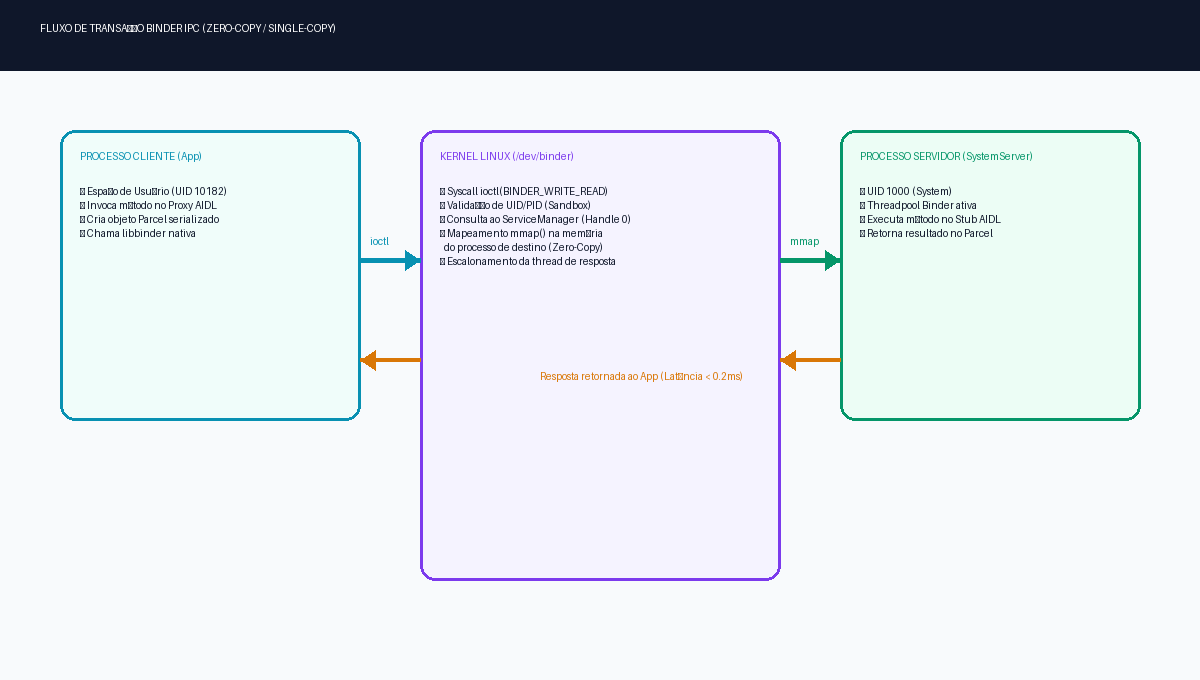
\includegraphics[width=0.95\textwidth]{imagens/fig_binder_ipc.png}
\caption{Fluxo Detalhado de Transação IPC no AOSP via driver \texttt{/dev/binder}: empacotamento em Parcel, syscall \texttt{ioctl}, resolução no ServiceManager e entrega Zero-Copy via \texttt{mmap} compartilhado.}
\label{fig:binder_flow_img}
\end{figure}

O cliente prepara uma estrutura de dados serializada chamada \texttt{Parcel}. Através da interface AIDL (\textit{Android Interface Definition Language}), o código Kotlin invoca um método local no \textit{Proxy}, que empacota os argumentos e realiza a chamada de sistema \texttt{ioctl(fd, BINDER\_WRITE\_READ, \&bwr)}. O kernel localiza a página de memória do processo destino pré-alocada via \texttt{mmap()} e grava os dados diretamente nela, acordando uma thread da threadpool do servidor para executar o \textit{Stub}.

\subsection{Observabilidade em Nanossegundos com Perfetto Trace}
\begin{figure}[htbp]
\centering
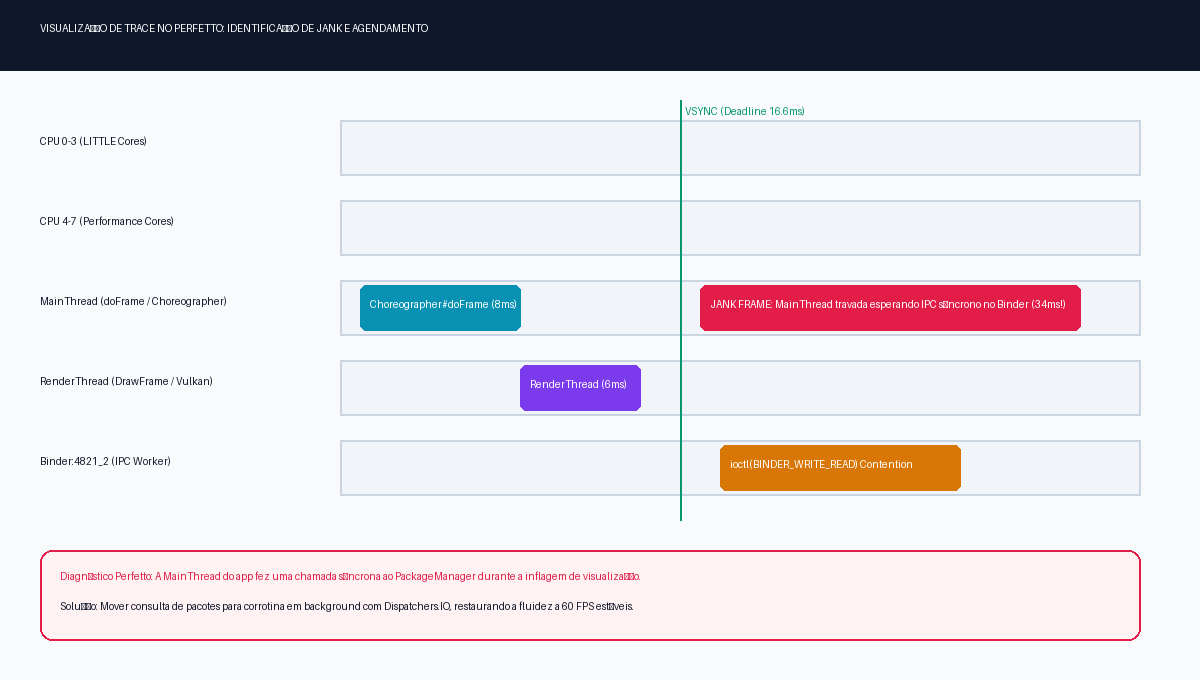
\includegraphics[width=0.95\textwidth]{imagens/fig_perfetto_timeline.png}
\caption{Rastreamento de Execução no Perfetto: identificação visual de contenção de lock no barramento Binder e diagnóstico de queda de quadros (\textit{jank frame}) violando o deadline de 16.6ms.}
\label{fig:perfetto_trace_img}
\end{figure}
Para diagnosticar gargalos que degradam a taxa de 60 ou 120 quadros por segundo (onde cada quadro dispõe de apenas $16{,}6\text{ ms}$ ou $8{,}3\text{ ms}$), utiliza-se o **Perfetto**:
\begin{itemize}
    \item Gravação de rastros baseada no subsistema \texttt{ftrace} do kernel;
    \item Eventos de agendamento de CPU: \texttt{sched\_switch} e \texttt{sched\_wakeup};
    \item Transações de Binder: visualização do tempo de espera e fila de atendimento;
    \item \textit{Choreographer} e \textit{RenderThread}: rastreamento de \texttt{doFrame}, inflamento de views e chamadas de desenho OpenGL/Vulkan.
\end{itemize}

---

\section{Aprendizado de Máquina e Aprendizado Profundo (30h)}

\begin{pedagogico}{Objetivo Pedagógico da Disciplina}
Capacitar os residentes a projetar, treinar e validar redes neurais profundas aplicadas à detecção de anomalias operacionais e predição de comportamento em sistemas Android, tratando dados ruidosos de telemetria.
\end{pedagogico}

\subsection{Detecção de Anomalias com Autoencoders Neurais}
Uma das aplicações de IA no AOSP é detectar quando um aplicativo entra em um estado anômalo de dreno silencioso de bateria ou vazamento de recursos. Para tal, treina-se um **Autoencoder** exclusivamente com dados de operação nominal:

\begin{equation}
    \mathbf{z} = \sigma(\mathbf{W}_e \mathbf{x} + \mathbf{b}_e) \quad \text{(Codificador)}
\end{equation}
\begin{equation}
    \hat{\mathbf{x}} = \sigma(\mathbf{W}_d \mathbf{z} + \mathbf{b}_d) \quad \text{(Decodificador)}
\end{equation}
onde $\mathbf{x} \in \mathbb{R}^d$ é o vetor de métricas instantâneas (uso de CPU por core, taxa de interrupts, frequência de chamadas IPC Binder). O modelo é treinado para minimizar o Erro Quadrático Médio de reconstrução (\textit{Reconstruction Error}):
\begin{equation}
    \text{MSE}(\mathbf{x}, \hat{\mathbf{x}}) = \frac{1}{d} \sum_{j=1}^{d} (x_j - \hat{x}_j)^2
\end{equation}

---

\section{IA On-device e Otimização de Modelos (20h)}

\begin{pedagogico}{Objetivo Pedagógico da Disciplina}
Dominar as técnicas de engenharia para adaptação de modelos neurais em dispositivos móveis, aplicando quantização afim de inteiros (INT8), poda esparsa de conexões sinápticas e delegação de tensores para a NPU via Android NNAPI e LiteRT.
\end{pedagogico}

\subsection{Teoria Matemática da Quantização Afim \texorpdfstring{(FP32 $\to$ INT8)}{(FP32 para INT8)}}
\begin{figure}[htbp]
\centering
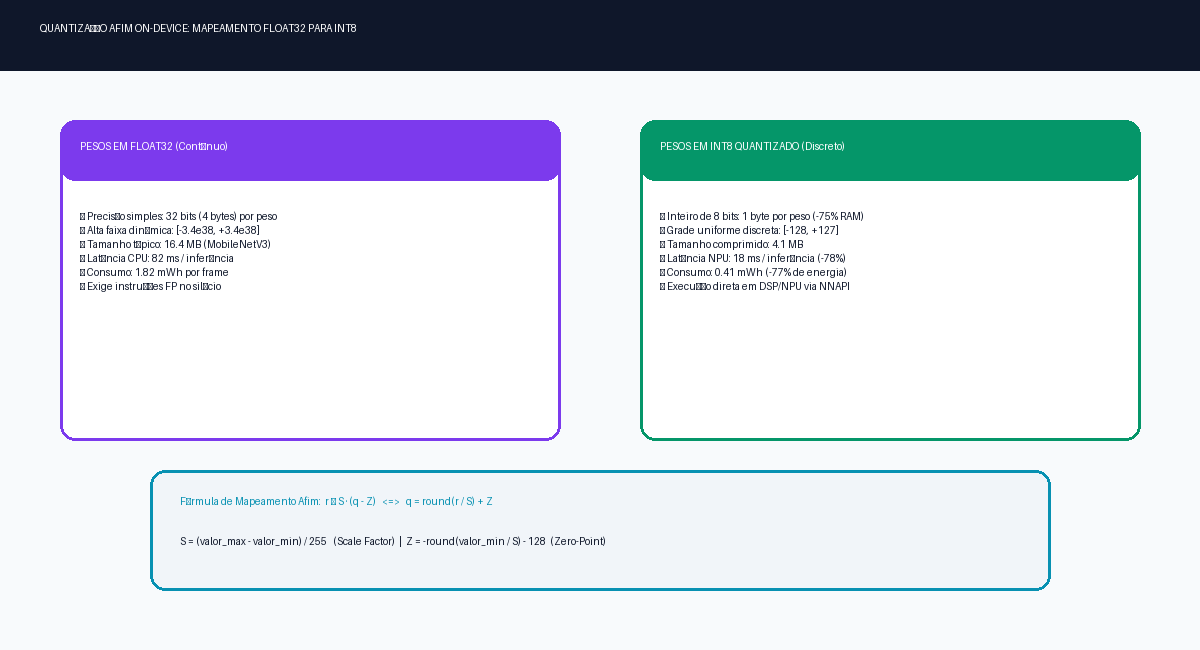
\includegraphics[width=0.95\textwidth]{imagens/fig_quantizacao_neural.png}
\caption{Mapeamento Afim de Quantização On-Device: conversão de tensores contínuos em Float32 para inteiros uniformes em INT8, exibindo redução de 75\% no tamanho e aceleração via NNAPI.}
\label{fig:quantizacao_img}
\end{figure}

Modelos neurais convencionais operam com tensores em ponto flutuante de precisão simples (\texttt{Float32}, ocupando 4 bytes por parâmetro). Em smartphones, essa representação consome banda excessiva de memória RAM e dissipa calor desnecessário.

A **Quantização Afim de Inteiros (Uniform Affine Quantization)** mapeia um valor real contínuo $r \in [\alpha, \beta]$ em um inteiro de 8 bits $q \in [-128, 127]$ através da relação linear:
\begin{equation}
    r \approx S \cdot (q - Z)
\end{equation}
onde $S = \frac{\beta - \alpha}{255}$ é o fator de escala e $Z = \text{round}\left( -\frac{\alpha}{S} \right) + q_{\text{min}}$ é o ponto zero.

---

\section{Revisão da Literatura e Estado da Arte: IA e Observabilidade em SO}

A literatura científica recente converge para a necessidade de observabilidade profunda com overhead desprezível e inferência inteligente descentralizada:
\begin{itemize}
    \item \textbf{Observabilidade em Kernel e Sistemas Operacionais:} \cite{gregg2019bpf} demonstra que ferramentas tradicionais baseadas em amostragem periódica de \texttt{/proc} introduzem distorções severas de amostragem (\textit{observer effect}). O uso de pontos de rastreamento estáticos (\textit{tracepoints}) e buffers circulares sem bloqueio no kernel Linux — como implementado no Perfetto — viabiliza capturar eventos em nanossegundos com consumo de CPU inferior a $1{,}5\%$.
    \item \textbf{Detecção Não-Supervisionada de Anomalias em Telemetria:} \cite{malhotra2016lstm} e \cite{zhou2017anomaly} comprovaram que redes neurais autoassociativas (Autoencoders e LSTM Encoder-Decoders) superam métodos estatísticos clássicos (como limites baseados em desvio padrão $\mu \pm 3\sigma$) na detecção de falhas silenciosas em séries temporais multidimensionais, pois aprendem correlações intrínsecas e não-lineares entre subsistemas heterogêneos.
    \item \textbf{Quantização com Aritmética de Inteiros Acelerada:} O trabalho seminal de \cite{jacob2018quantization} estabeleceu as bases formais da quantização afim adotada pelo Google no ecossistema Android/LiteRT, comprovando que a substituição de instruções de ponto flutuante por aritmética de inteiros INT8 com multiplicadores de ponto fixo reduz em $75\%$ o consumo de largura de banda de memória e acelera em mais de $4\times$ a execução em aceleradores de hardware como NPUs e DSPs, preservando mais de $99\%$ da acurácia original de redes complexas como MobileNet.
\end{itemize}

---

\section{Arquitetura de Engenharia do Projeto Final: Seldon Anomaly Watcher}

Como projeto final de conclusão do Módulo 2, os residentes projetam e implementam o **Seldon Anomaly Watcher**, uma solução completa de governança inteligente embarcada no AOSP.

\begin{figure}[htbp]
\centering
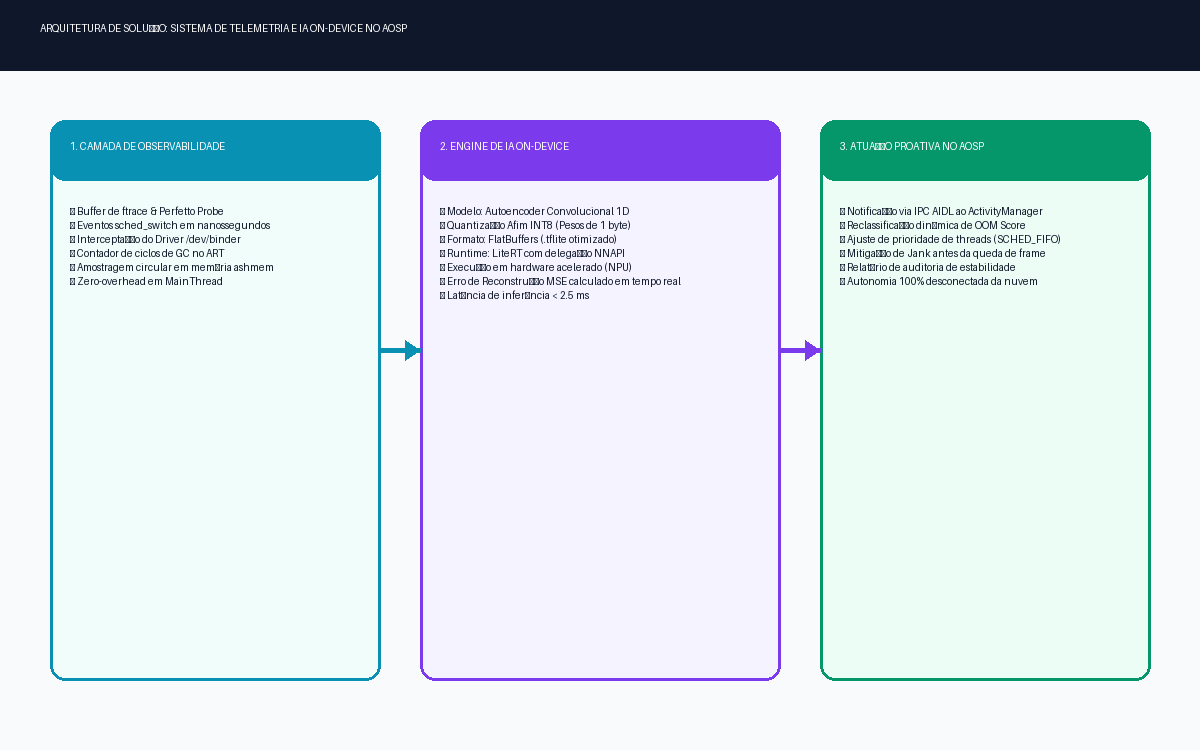
\includegraphics[width=0.95\textwidth]{imagens/fig_arq_projeto_ia.png}
\caption{Arquitetura de Engenharia do Projeto Final (Módulo 2): Pipeline completo desde a captura de telemetria no kernel via Perfetto até a inferência quantizada em NPU e atuação corretiva no System Server.}
\label{fig:arq_ia_projeto}
\end{figure}

\subsection{Especificação Técnica dos Módulos da Solução}
A arquitetura estrutura-se em três subsistemas desacoplados:
\begin{enumerate}
    \item \textbf{Coletor de Telemetria de Baixo Nível (Kernel Probe):}
    \begin{itemize}
        \item Consome dados de \texttt{tracefs} e eventos \texttt{sched\_switch}, calculando a duração das fatias de tempo (\textit{timeslices}) de cada thread em execução;
        \item Monitora transações no driver \texttt{/dev/binder}, registrando tempos de espera síncronos e tamanho dos buffers transmitidos;
        \item Grava vetores de atributos em janelas deslizantes de $500\text{ ms}$ em memória compartilhada (\textit{ashmem}).
    \end{itemize}
    \item \textbf{Engine de Inferência On-Device (LiteRT + NNAPI):}
    \begin{itemize}
        \item Executa o modelo Autoencoder Convolucional 1D quantizado em INT8 (\texttt{anomaly\_detector\_v2.tflite});
        \item Delegado via driver Android NNAPI diretamente para a NPU do chipset;
        \item Computa o erro de reconstrução instantâneo $\text{MSE}_t$; se $\text{MSE}_t > \tau_{\text{critico}}$, dispara um evento de anomalia estruturado.
    \end{itemize}
    \item \textbf{Atuador Proativo de Políticas AOSP (System Server Handler):}
    \begin{itemize}
        \item Recebe o alerta via interface AIDL \texttt{ISeldonPolicyCallback};
        \item Reclassifica preventivamente a prioridade de agendamento de threads com risco de jank de \texttt{SCHED\_OTHER} para \texttt{SCHED\_FIFO};
        \item Notifica o \texttt{ActivityManagerService} para contenção de tarefas em segundo plano causadoras de concorrência excessiva de locks.
    \end{itemize}
\end{enumerate}
